\subsection*{2.1}
  % Implement the CE-CC amplifier shown below:
    \begin{figure}[h!]
        \centering
        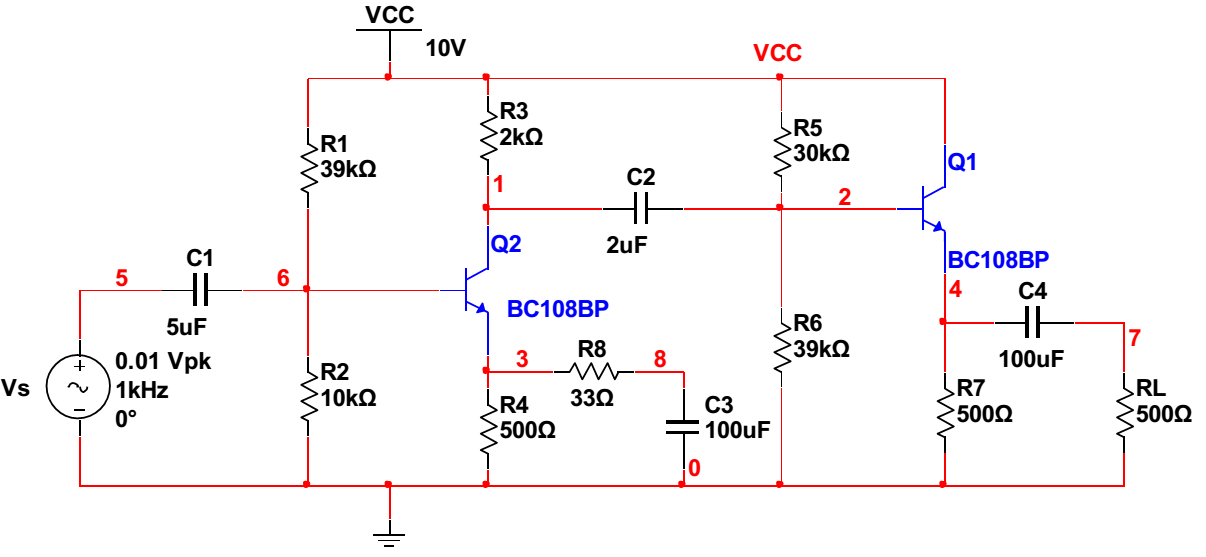
\includegraphics[width=13cm]{fig2-1.png}
        \captionof{figure}{The CE-CC amplifier to be implemented in Task 2.1}
    \end{figure}    

Figure 9 was implemented in $MultiSim$.

\subsection*{2.2}
  % Using  proper  simulation  techniques,  determine  the  following  parameters  of  the  circuit:
  \subsection*{(i) Midband voltage gain}

	\begin{figure}[h]
        \centering
        \begin{subfigure}[h]{0.7\textwidth}
                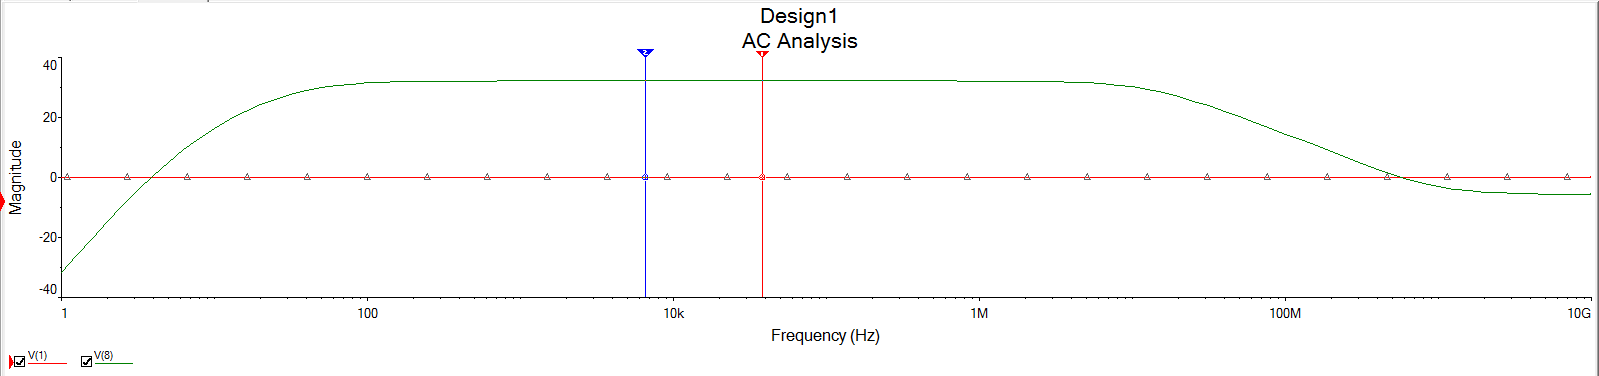
\includegraphics[width=\textwidth]{Task2_1A.png}
                \label{fig:HJÖRLEIFUR}
        \end{subfigure}
        \begin{subfigure}[h]{0.25\textwidth}
                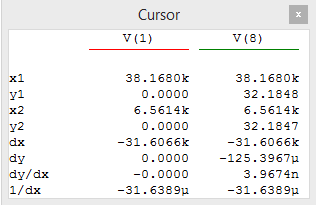
\includegraphics[width=\textwidth]{Task2_1B.png}
                \label{fig:LÁRUS}
        \end{subfigure}
        \caption{figure}{AC analysis of circuit in figure 9:Finding the midband gain}
	\end{figure}

    By using results from the AC analysis as seen in figure 10 to determine the midband gain in decibel and convert over to voltage gain($\frac{V}{V}$):

   	From figure 10 hence the midband gain:
   	$$ V_{0} = 32.1848 \ dB $$ 

   	$$ 20 \cdot log{\ A_{M}} = 32.1848 dB \rightarrow A_{M} = 40.66\  \frac{V}{V} $$



	\subsection*{(ii) Input resistance}
    \begin{figure}[h!]
        \centering
        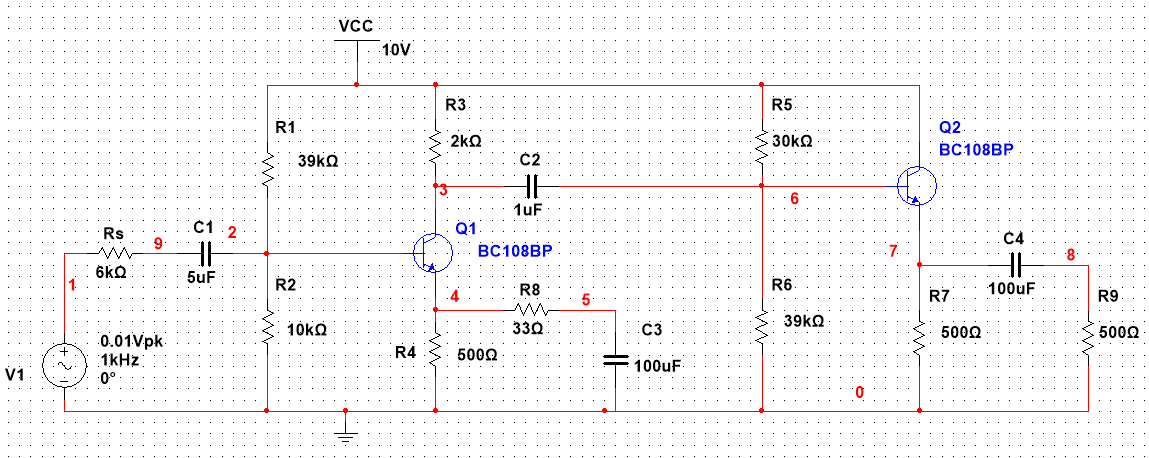
\includegraphics[width=13cm]{Task2_2C.png}
        \captionof{figure}{CE-CC circuit with $R_{s}$}
    \end{figure}  

	\begin{figure}[h]
        \centering
        \begin{subfigure}[h]{0.7\textwidth}
                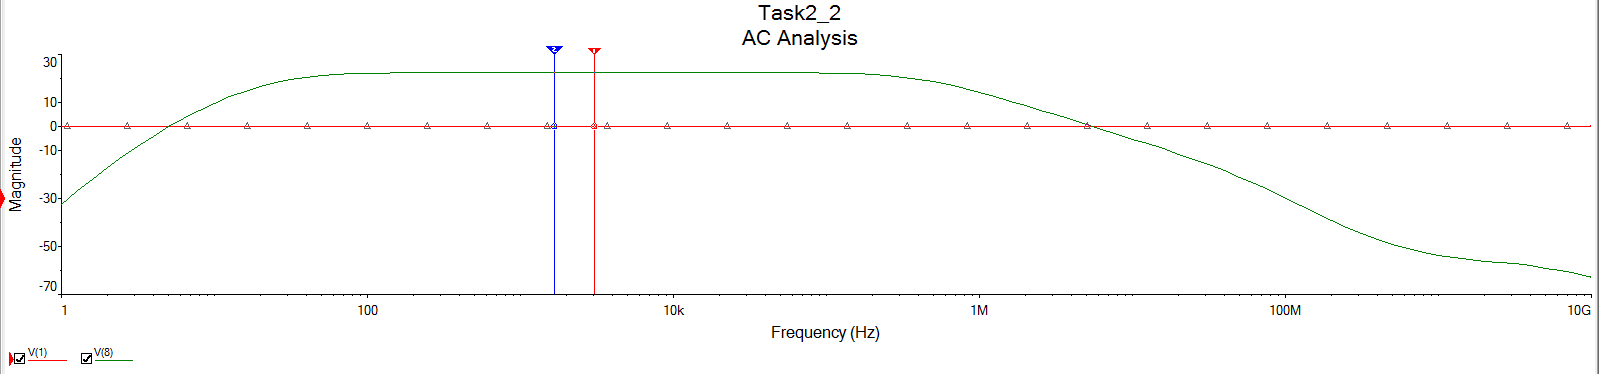
\includegraphics[width=\textwidth]{Task2_2A.png}
                \label{fig:}
        \end{subfigure}
        \begin{subfigure}[h]{0.25\textwidth}
                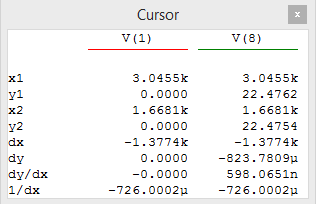
\includegraphics[width=\textwidth]{Task2_2B.png}
                \label{fig:}
        \end{subfigure}
        \caption{figure}{AC analysis of circuit in figure 11}
	\end{figure}

	By adding a $R_{s}$ in the circuit as seen in figure 11,  and find the midband gain of the circuit with AC analysis as seen in figure 12:
	$$ 20 \cdot log(A_{M2}) = 25.2002 dB  \rightarrow A_{M3} = 18.19 \frac{V}{V} $$
	By using results from Task2.2.i that the midband gain without $R_{s}$ is $A_{M1} = 40.66 \frac{V}{V}$ and the formula for midband gain with $R_{s}$ is:

	$$ A_{M2} = A_{M1} \cdot \frac{R_{in}}{R_{in} + R_{s}} \rightarrow R_{in} = \frac{R_{s}}{\frac{A_{M1}}{A_{M2}}-1} $$
	
	$$R_{in} = \frac{6\ kHz}{\frac{40.66}{18.19}-1} = 4857.14 \Omega \ $$ 
	\pagebreak

 	\subsection*{(iii) Output resistance}

	\begin{figure}[h!]
	    \centering
	    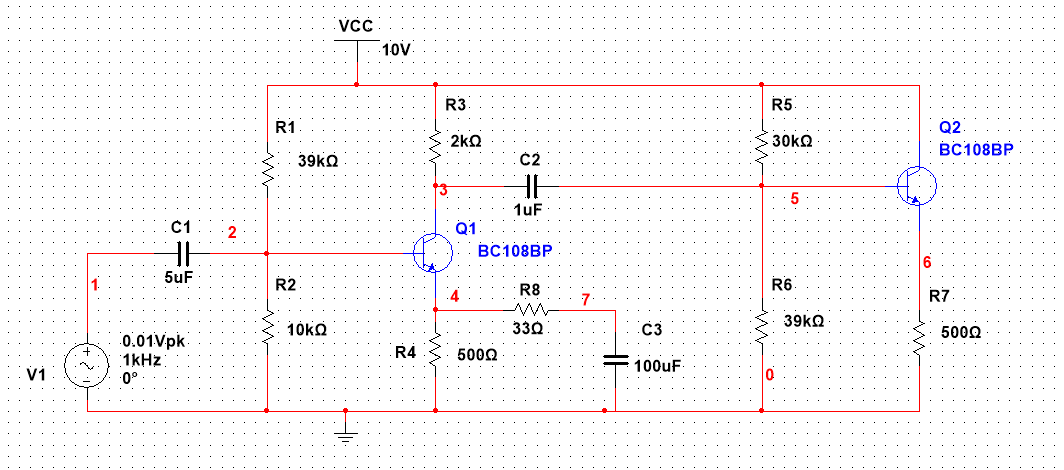
\includegraphics[width=13cm]{Task2_3C.png}
	    \captionof{figure}{CE-CC circuit without the $R_{L}$}
	\end{figure}  \

	\begin{figure}[h]
	    \centering
	    \begin{subfigure}[h]{0.7\textwidth}
	            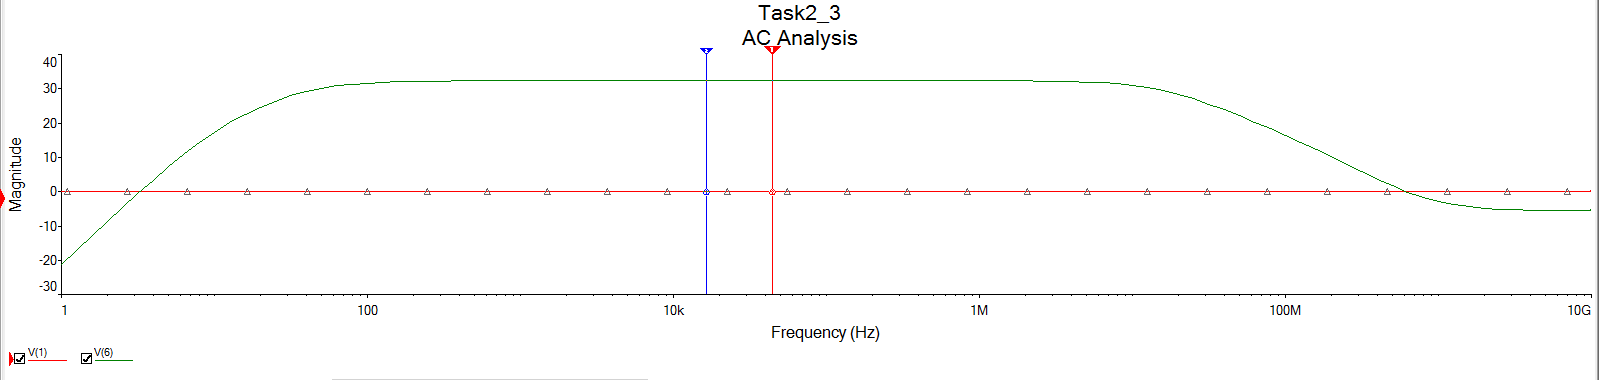
\includegraphics[width=\textwidth]{Task2_3A.png}
	            \label{fig:}
	    \end{subfigure}
	    \begin{subfigure}[h]{0.25\textwidth}
	            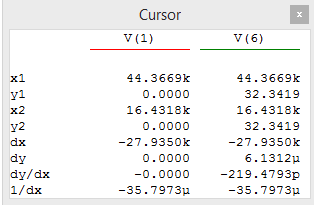
\includegraphics[width=\textwidth]{Task2_3B.png}
	            \label{fig:}
	    \end{subfigure}
	    \caption{figure}{AC analysis of circuit in figure 13}
	\end{figure}

	By removing the load resistor and finding the midband gain in the circuit from AC analysis as seen in figure 14.

	$$ 20 \cdot log(A_{M3}) = 32.3419 dB  \rightarrow A_{M3} = 41.40 \frac{V}{V}$$


	By using result from Task2.2.i the midband gain with $R_{L}$ is $A_{M1} = 40.66$ and the formula for midband gain without $R_{L}$ is:

	$$A_{M1} = A_{M3} \cdot \frac{R_{L}}{R_{L} + R_{out}} \rightarrow R_{out} = R_{L} \cdot (\frac{A_{M3}}{A_{M1} - 1})  $$
	$$R_{out} = 500 \cdot (\frac{41.40}{40.66}-1) = 9.10\ \Omega$$ 

	\pagebreak


	\subsection*{(iv) Lower 3dB frequency}

	\begin{figure}[h!]
	    \centering
	    \begin{subfigure}[h]{0.7\textwidth}
	            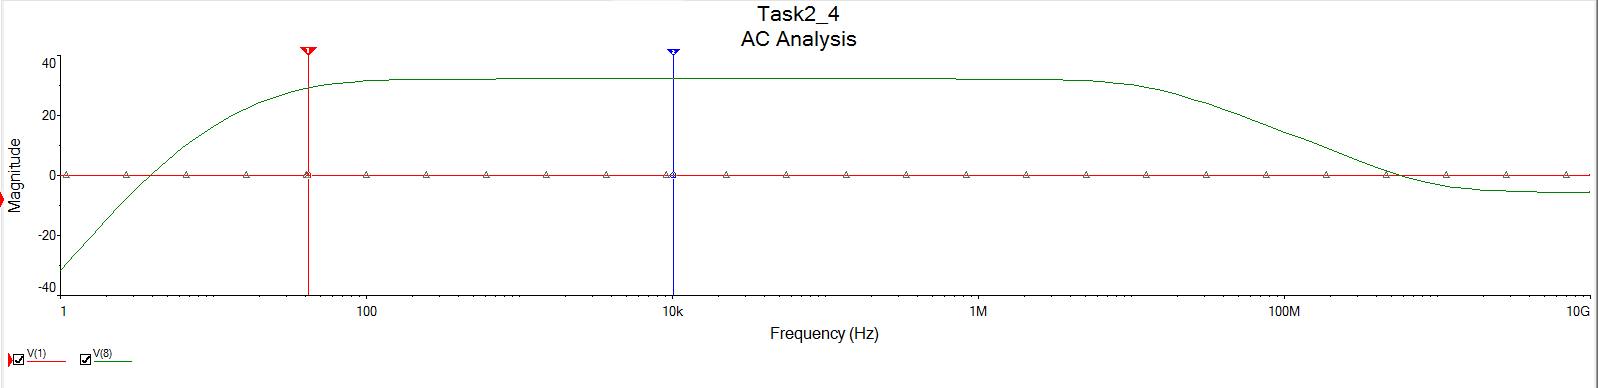
\includegraphics[width=\textwidth]{Task2_4A.png}
	            \label{fig:}
	    \end{subfigure}
	    \begin{subfigure}[h]{0.25\textwidth}
	            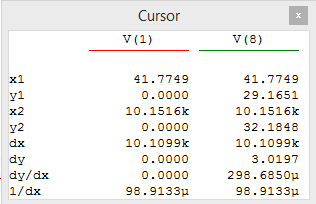
\includegraphics[width=\textwidth]{Task2_4B.png}
	            \label{fig:}
	    \end{subfigure}
	    \caption{figure}{AC analysis of circuit in figure 9}
	\end{figure}

	To find the lower 3 dB frequency by finding the 3 db drop to the left from the midband gain as seen in figure 9.

	$$f_{L} =  41.15 Hz$$




	
	\subsection*{(v) Upper 3dB frequency}

	\begin{figure}[h!]
	    \centering
	    \begin{subfigure}[h]{0.7\textwidth}
	            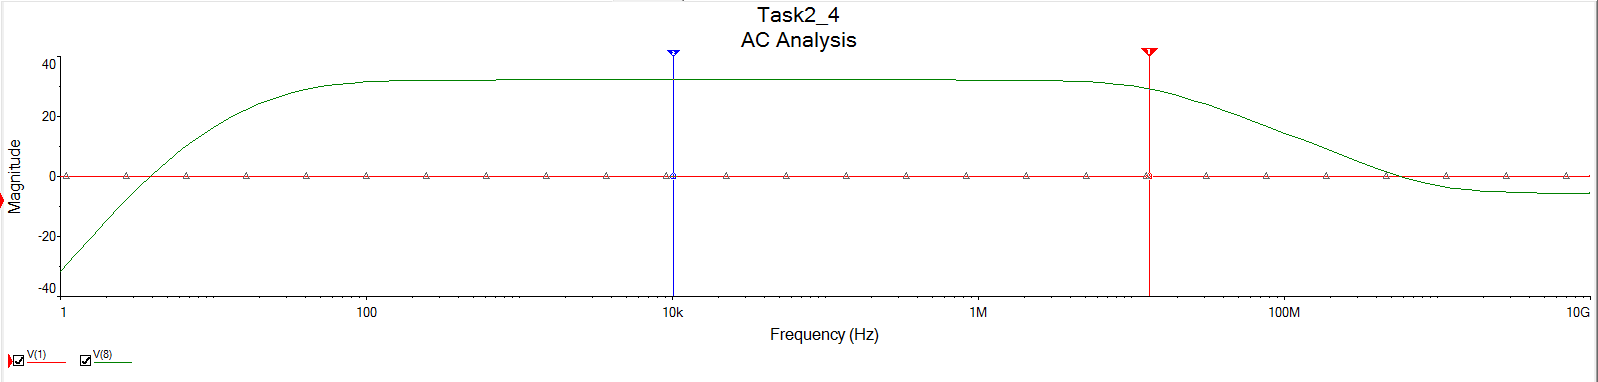
\includegraphics[width=\textwidth]{Task2_5A.png}
	            \label{fig:}
	    \end{subfigure}
	    \begin{subfigure}[h]{0.25\textwidth}
	            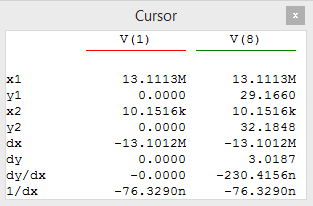
\includegraphics[width=\textwidth]{Task2_5B.png}
	            \label{fig:}
	    \end{subfigure}
	    \caption{figure}{AC analysis of circuit in figure 9}
	\end{figure}
	To find the higher 3 dB frequency by finding the 3 db drop to the right from the midband gain as seen in figure 9.

	$$f_{H} = 13.11 \ M Hz $$
\pagebreak
  \subsection*{(vi) Output voltage when total harmonics distortion (THD) < 5\%}
  % In order to evaluate the THD in the circuit, a fourier analysis has to be done. The input voltage is lowered gradually from 0.01 V until the THD is lower than 5\%. When that value was reached for the THD the Output voltage was determined 2.5471 V and the input voltage was then at 0.0731 V.

  In order to evaluate the THD in the circuit seen in figure 9, a fourier analysis was done in $MultiSim$. The maximun output voltage was found to be 2.55 V when the THD was less than 5 $\%$ as seen in figure 17. The maxmimum output voltage was found by increasing the input voltage without going over the 5$\%$ THD. The input voltage was 0.67 V	


	\begin{figure}[h!]
        \centering
        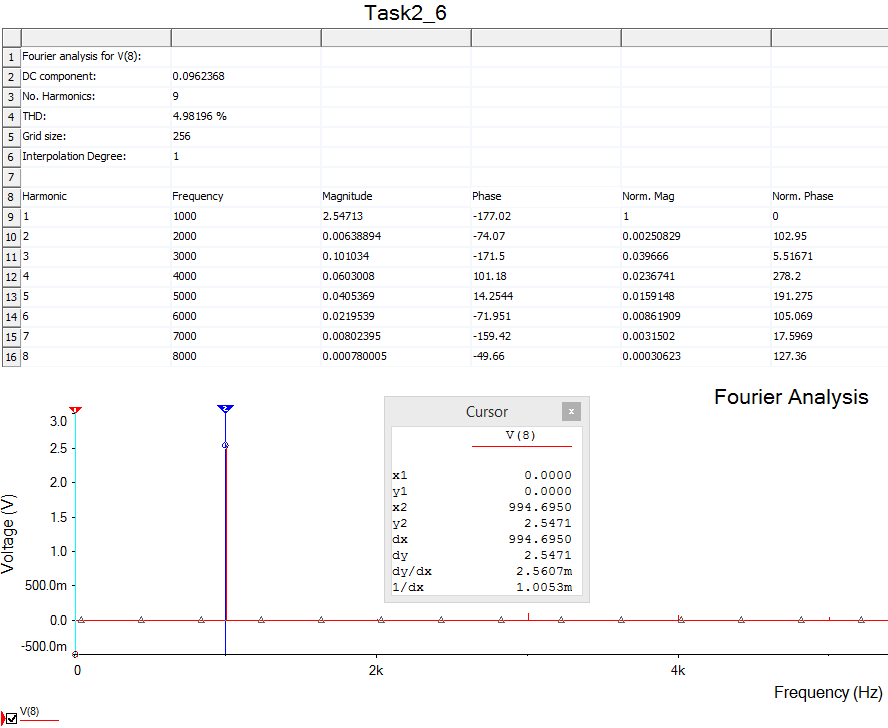
\includegraphics[width=16cm]{Task2_6_MaxOutPutVoltage.png}
        \captionof{figure}{The fourier analysis with THD $\approx$ 5\%}
	\end{figure}
    
\pagebreak
  
\subsection*{2.3}
  % Summarize  the  circuit  parameters  in  a  table  and  attach  relevant  plots.  Explain  the
  % simulation techniques that you exploited.
  
	\begin{table}[htbp]
     \centering
       \begin{tabular}{c|c}
        \hline
         Circuit Parameters & Values \\
       \hline
        Midband voltage gain          & 40.66 $\frac{V}{V}$ \\
        Input Resistance & 4857.14\ $\Omega$ \\
        Output Resistance & 9.18 $\Omega$\\
        Lower 3dB frequency & 41.15 \ Hz\\
        Higher 3dB frequency & 13.11\ MHz\\
        Maximum Output Voltage & 2.55 V\\
       \end{tabular}%
     \caption{Result from simulation for CE-CC amplifier.}
     \label{tab:addlabel}%
	\end{table}%